\chapter{Driver commande des moteurs}

\section{Introduction}
Un driver est un programme développé avec un language reconnu pour sa proximité avec le matériel, le language C. Et c'est la raison d'être des drivers. Ces derniers font la passerelle entre les applications qui se trouvent dans la partie utilisateur (user-space) et le matériels. \newline Le plus simple des exemples est celui du clavier. Lorsque j'appuis sur une touche pour écrire ce rapport un contact électrique est émit et informe le micro-processeur qu'une touche à été appuyé. Puis un programme, dit driver-souris, viens contrôller les entrées pour savoir quelle touche a été pressé. Et envoi cette information au système d'exploitation pour que la lettre soit affichée.\newline 
Le driver moteur a pour mission de permettre de contrôler les moteurs de rotation, inclinaison et zoom du télescope. D'informer le logiciel principal de l'accomplissement d'une manoeure, théoriquement (explication chapitre 10.2). Il assure la sécurité du système de pilotage à bas niveau. Le système de sécurité consiste à interrompre le mouvement d’inclinaison ou de zoom si ils atteignent leur fin de course.

\section{Fonctionnalités du driver}

\begin{figure}[H]
    \centering
    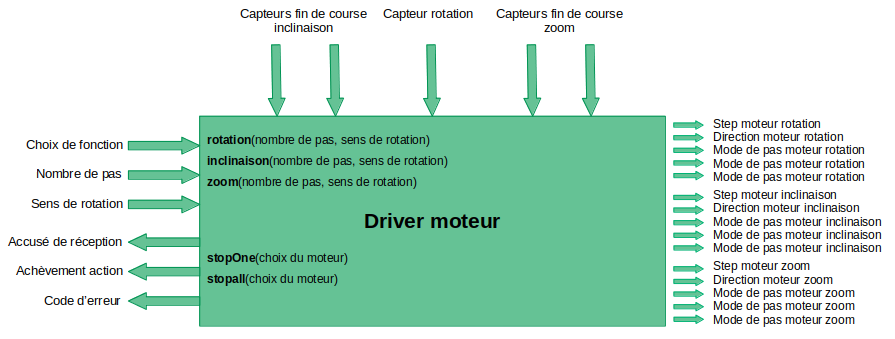
\includegraphics[width=1\linewidth]{\figures/illustration_entree_sortie_driver_moteur.png}
    \decoRule
    \caption[
    Schéma des entrées / sorties du driver moteur]{
    Schéma des entrées / sorties du driver moteur}
    \label{fig:Schéma des entrées / sorties du driver moteur}
    \end{figure}

\vspace{1cm}

La figure 9.1 représente le driver contrôlant les moteurs. À gauche du block il y a les entrées du driver, se sont les données que attent le driver pour entreprendre une action. \newline 2 exemples: 
\begin{itemize}
	\item Faire tourner le zoom de 50 pas de droite à gauche:
	\begin{enumerate}
		\item Envoi au driver les nombres 3 ; 50 ; 0 pour choisir la fonction zoom, nombre de pas, sens de rotation droite à gauche;
		\item Reception de l'accusé de réception contenant les nombres 3 ; 50 ; 0 ;
		\item Reception de l'achèvement d'action contenant le nombre 1.
	\end{enumerate}
	\item Arreter tout les moteurs
	\begin{enumerate}
		\item Envoi au driver le nombre 5 pour choisir la fonction stopall
		\item Reception de l'accusé de réception contenant le nombre 5;
		\item Reception de l'achèvement d'action contenant le nombre 1.
	\end{enumerate}
\end{itemize}

\begin{figure}[H]
    \centering
    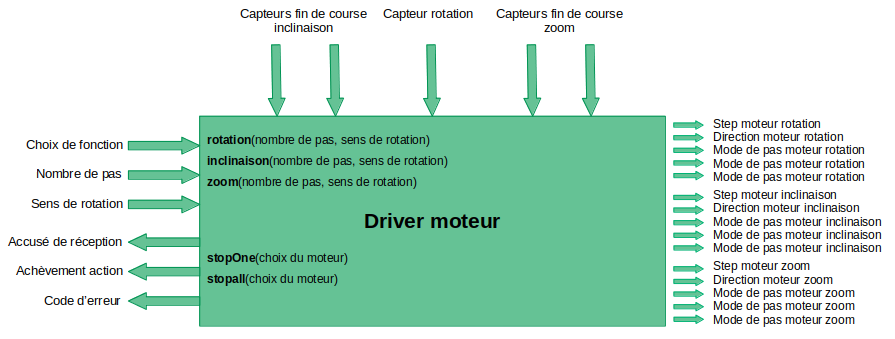
\includegraphics[width=1\linewidth]{\figures/illustration_entree_sortie_driver_moteur.png}
    \decoRule
    \caption[
    Schéma des entrées / sorties du driver moteur]{
    Schéma des entrées / sorties du driver moteur}
    \label{fig:Schéma des entrées / sorties du driver moteur}
    \end{figure}

Une fois une manoeuvre terminé le driver informe l'application principale que l'action demandé est arrivé à son terme. Cependant d'un point de vue driver moteur il y a pas de possibilité de vérifier si le télescope est bien placer là où on lui a demander de ce placer. Si une personne ou objet block le mouvement du telescope ou des moteurs ces derniers ne renvairons pas d'avertissement. C'est dont la centrale inertielle qui contrôlera le bon placement du télescope. \newline
Les capteurs de fin de course servent de sécurité, cette partie est indépendante du reste. Elle a pour but d'arrêter un moteur qui à atteint sa position maximale, hormis pour le capteur de rotation qui à pour utilité dans un premier temps de faire une interruption lorsque un tour complet. \newline Avec cette information on pourra déterminer le nombre de pas moteur qu'il faut faire pour faire un tour complet de télescope sur lui même. Et dans un second temps de donner un point de repère pour les recalibrages de la centrale inertielle. \newline 
Les sorties "Mode de pas moteur..." permettent de choisir dans quel mode de rotation doit tourner le moteur (pas complet, demi-pas, quart de pas, huitième de pas, seizième de pas). Augmenter la division de pas permet d’affiner la rotation afin d’atteindre l’angle le plus exact possible à ce qui à été commandé. Ainsi lorsqu'un moteur a accomplie environ 90\% de la distance à réalisé, on change le mode de pas afin d'arriver au plus proche de l'angle exacte.   



\section{Interactions avec le driver}

Le driver devra pourvoir être utilisé à partir d'une application situé dans le user-space du linux embarqué. Pour cela j'ai étudié et testées plusieures solutions. \newline
La première qui m'est venu à l'idée était d'utiliser l'IPC (inter process communication). \newline
Une seconde plus archaïque m'est venu à l'idée, celle de partager un ficher entre le programme dans le user-space et du driver. Pour que le programme dans le user-space puisse transférer ses ordres. Cependant je trouve cette solution pas très sécuritaire. \newline
La troisième solution qui m'a été proposé par Vincent Poulailleau est d'utiliser la fonction ioctl. C'est cette solution que j'ai retenu car elle est une technique très rodé dans le domaine car elle était déjà utilisé à la version 7 d'UNIX. 
\vspace{1cm}

\section{Validation des fonctionnalitées de bases}

\section{Câblage}
\begin{figure}[H]
    \centering
    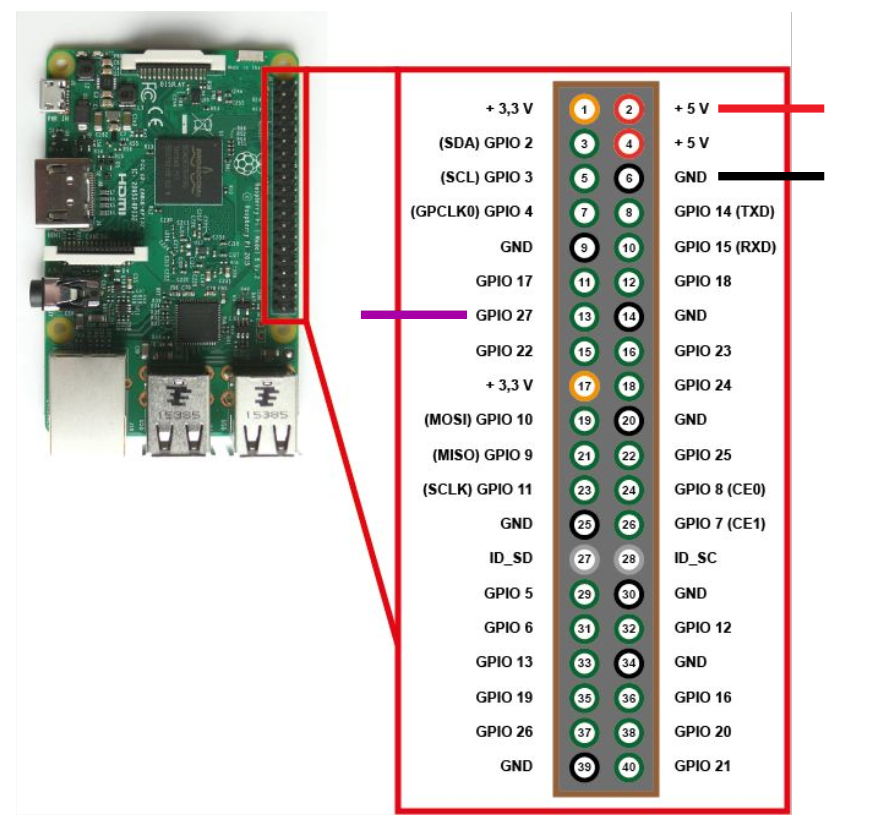
\includegraphics[width=0.5\linewidth]{\figures/sch_pinout.png}
    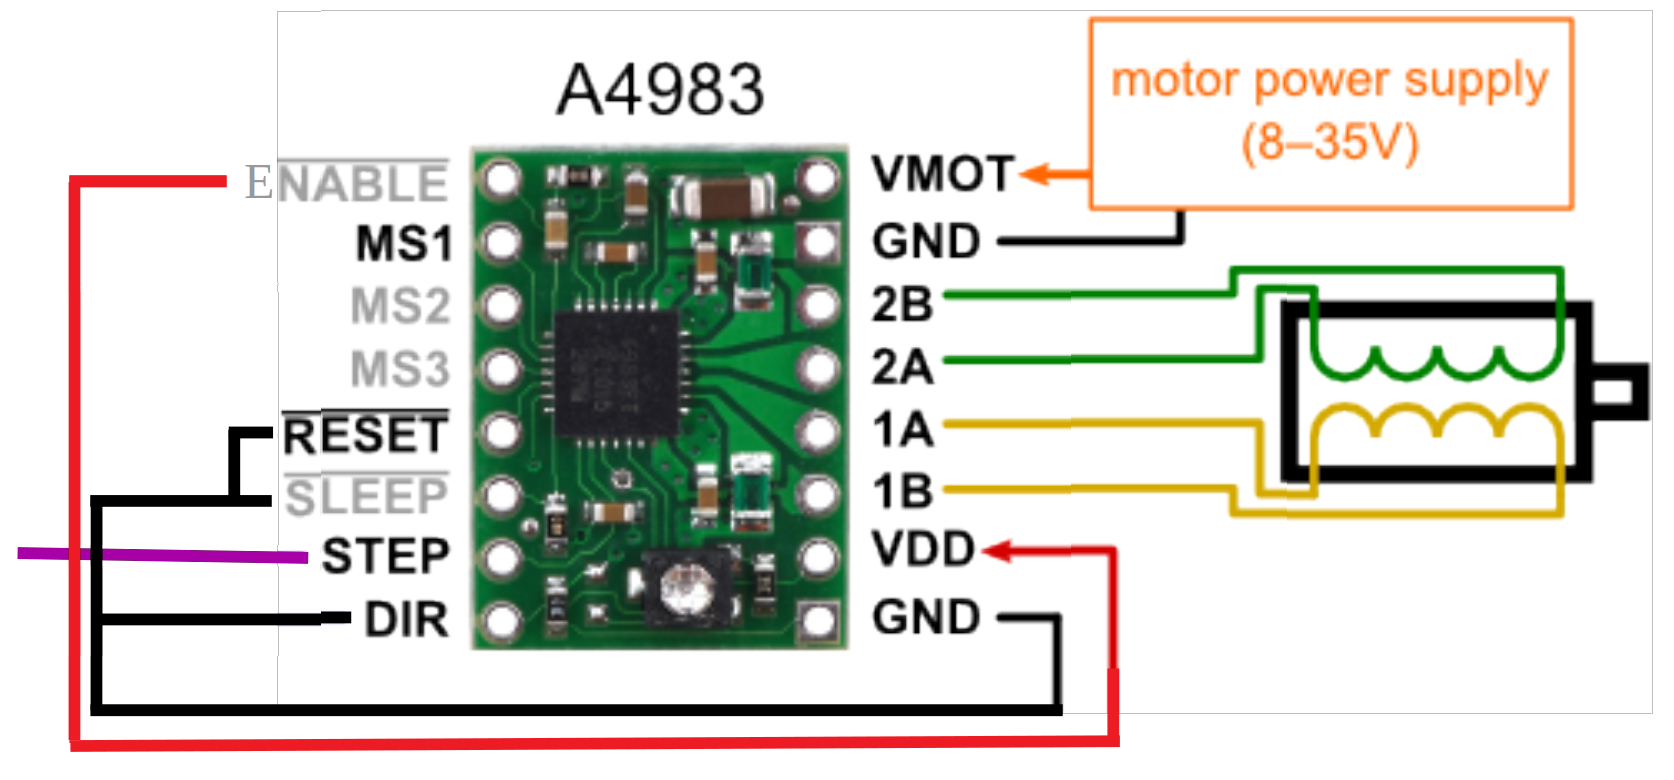
\includegraphics[width=0.5\linewidth]{\figures/sch_a4983.png}
    \decoRule
    \caption[
    Schéma de câblage d'un contrôleur moteur sur la Raspberry Pi]{
    Schéma de câblage d'un contrôleur moteur sur la Raspberry Pi}
    \label{fig:Schéma de câblage d'un contrôleur moteur sur la Raspberry Pi}
    \end{figure}

\vspace{1cm}

Pour valider mon driver, je l’ai testé avec une Raspberry Pi, un contrôleur moteur et un moteur.

\begin{figure}[H]
    \centering
    \includegraphics[width=0.9\linewidth]{\figures/photo_test_motor.jpg}
    \decoRule
    \caption[
    Photo du banc de test]{
	Photo du banc de test}
    \label{fig:Photo du banc de test}
    \end{figure}

\vspace{1cm}

J’ai pu valider les fonctionnalités développées, cependant la vitesse max atteinte par le moteur contrôlé par le driver est inférieure à celle que l'on peut atteindre en contrôlant le moteur avec un générateur basse fréquence.
Voici le résultat de la commande envoyée par la Raspberry Pi par la pin Step au contrôleur moteur pour faire avancer à chaque front montant le moteur de 1 pas.

\begin{figure}[H]
    \centering
    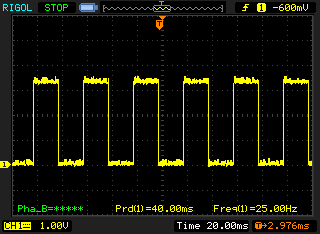
\includegraphics[width=0.5\linewidth]{\figures/osc_motor.png}
    \decoRule
    \caption[
    Mesure à l'oscilloscope de la commande moteur générée]{
	Mesure à l'oscilloscope de la commande moteur générée}
    \label{fig:Mesure à l'oscilloscope de la commande moteur générée}
    \end{figure}

\vspace{1cm}

Après avoir étudié les résultats avec d'autres professeurs, j'ai conclu que la période minimale que je puisse atteindre soit de $20ms$ est normal. Cette limitation est due au fait que mon driver n'a pas la priorité des ressources dans le Linux. Et que le Linux a un cycle lecture/écriture des entrées/sorties limité. Pour améliorer cela il faudrait passer sur un Linux temps réel.


